\section{Описание задачи}
Данная курсовая работа выполнена в раках проекта по разработке мобильного устройства  на платформе Raspberry Pi Zero~\cite{RPiZero}. Данный проект включает в себя несколько задач:
\begin{itemize}
\item разработка аппаратной платформы мобильного устройства на основе Raspberry Pi Zero --- подбор необходимых компонентов мобильного устройства (GSM модуль, динамик, микрофон, аккумулятор и т.д.) и их размещение на плате устройства
\item установка и конфигурирование ОС для Raspberry Pi
\item разработка стека драйверов для комплектующих
\item разработка сервисного слоя (в виде демонов UNIX), который будет предоставлять необходимую информацию клиентским приложениям
\item \textbf{разработка мобильного оконного менеджера}, который позволит запускать и отображать на экране графические пользовательские приложения
\item разработка клиентских приложений (для осуществления звонков, настроек и т.д.)
\end{itemize}

Архитектура разрабатываемого проекта приведена на рисунке~\ref{fig:architecture}.
\begin{figure}[h!]
\center{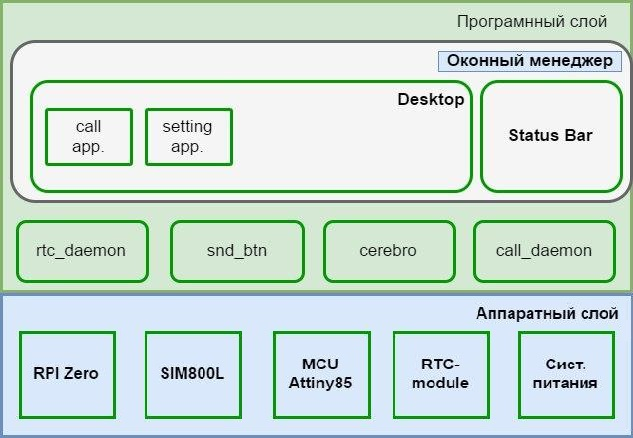
\includegraphics[width=\linewidth]{architecture}}
\caption{Архитектура проекта}
\label{fig:architecture}
\end{figure}

Таким образом, конечной целью разработки оконного менеджера~(ОМ) является его запуск на Raspberry Pi Zero. Необходимо учесть, что Raspberry обладает малой вычислительной мощностью, поэтому ОМ должен быть реализован как можно более оптимальным образом.

Мобильный ОМ должен так же иметь два встроенных системных приложения:
\begin{itemize}
\item строка состояния, которая отображает информацию об устройстве (текущее время, уровень заряда, уровень сигнала и т.д.). Строка состояния всегда отображается в верхней части экрана
\item рабочий стол, на котором расположены иконки запуска приложений, установленных в системе. Рабочий стол отображается на всю часть экрана, не занятую строкой состояния
\end{itemize}
Данные системные приложения не являются непосредственной частью ОМ. ОМ автоматически запускает их при своем запуске, и запоминает их идентификаторы для соответствующего отображения. ОМ должен иметь возможности указания путей к приложениям строки состояния и рабочего стола (т.е. должен иметь возможность конфигурирования).

При запуске несистемных приложений ОМ скрывает рабочий стол, выводит запущенное приложение на передний план и делает его активным. ОМ должен поддерживать три типа окон:
\begin{itemize}
\item обычные окна приложений, которые отображаются во весь экран
\item всплывающие уведомления (например, контекстное меню при нажатии правой кнопки мыши), которые отображаются в соответствии со своими размерами в указанной точке. Например, при нажатии на правую кнопку мыши открывается контекстное меню в точке нажатия с необходимыми размерами
\item окна меню (например стандартные меню типа "Файл" и т.д. в верхней части приложений). Должны запускаться в соответствии со своими размерами и отрисовываться начиная с нажатой кнопки.
\end{itemize}

Созданный оконный менеджер так же должен иметь возможность обработки управляющих комбинаций клавиш для:
\begin{itemize}
\item закрытия приложения
\item завершения работы ОМ
\item перелистывания окон
\item запуска терминала
\end{itemize}

Так же ОМ должен иметь возможности перемещения и изменения размеров окон.